\documentclass[12pt, a4paper]{article}

\usepackage{indentfirst}
\usepackage{graphicx}
\usepackage{amsmath}
\usepackage[T1]{fontenc}
\usepackage{listings}
\usepackage{xcolor}
\usepackage{pgfplots}
% Margin
\usepackage[margin=1.2in]{geometry}
%

% caption redefinitions
\renewcommand{\figurename}{Slika}
\renewcommand{\lstlistingname}{Kod}
%

% code settings
\definecolor{codegreen}{rgb}{0,0.6,0}
\definecolor{codegray}{rgb}{0.5,0.5,0.5}
\definecolor{codepurple}{rgb}{0.58,0,0.82}
\definecolor{backcolour}{rgb}{0.95,0.95,0.92}

\lstdefinestyle{mystyle}{
	language=C++,
	backgroundcolor=\color{backcolour},   
	commentstyle=\color{codegreen},
	keywordstyle=\color{magenta},
	numberstyle=\tiny\color{codegray},
	stringstyle=\color{codepurple},
	basicstyle=\ttfamily\footnotesize,
	breakatwhitespace=false,         
	breaklines=true,                 
	captionpos=b,                    
	keepspaces=true,                 
	numbers=left,                    
	numbersep=5pt,                  
	showspaces=false,                
	showstringspaces=false,
	showtabs=false,                  
	tabsize=2
}

\lstset{style=mystyle}
%

%opening
\title{Paralelizacija genetskog algoritma za problem\\N - kraljica}
\author{Vladimir Popov\\Balša Bulatović}
\date{Jun, 2023}

\begin{document}
	
	% Naslovna
	\maketitle
	\thispagestyle{empty}
	\newpage
	\
	\thispagestyle{empty}
	\newpage
	%
	
	% Sadrzaj
	\renewcommand{\contentsname}{Sadržaj}
	\tableofcontents
	\thispagestyle{empty}
	\cleardoublepage
	\newpage
	\
	\thispagestyle{empty}
	\newpage
	%
	
	\setcounter{page}{1}
	
	\section{Opis problema}
	Problem N - kraljica predstavlja klasičan kombinatorni problem u oblasti računa\-rstva. Problem ima jednostavnu strukturu i definisan je na sledeći način. Na šahovsku tablu, veličine $N \times N$, treba postaviti $N$ kraljica, tako da se nijedan par kraljica medjusobno ne napada. Dve kraljice se napadaju ukoliko se nalaze u istom redu, koloni ili na dijagonali (Slika 1).
	
	\begin{figure}[!htb]
		\begin{center}
			\includegraphics[width=0.5\textwidth]{images/queen-moves.png}
			\caption{Kretanje kraljice u šahu}
		\end{center}
	\end{figure}
	
	Najjednostaviji primer ove vrste problema, za koji postoji rešenje, predstavlja problem 4 kraljice. U opštem slučaju, postoji $\dbinom{n^2}{n}$ različitih načina da se postavi N kraljica na tablu veličine $N \times N$, tako da za relativno mali problem od 10 kraljica postoji više od $1.73 * 10^3$ mogućnosti, što predstavlja velik prostor rešenja za pretraživanje, kod tako malog problema.
	
	\newpage
	
	\section{Osnovne karakteristike i serijska implementacija algoritma}
	Zarad rešavanja gorepomenutog problema, odlučili smo se za pristup genetskog algoritma. Njegovo generalno funkcionisanje, kao i konkretna implementacija za ovaj problem biće objašnjeni u narednim potpoglavljima.
	
	\subsection{Prikaz jedinke}
	Temelj svakog genetskog algoritma jesu jedinke, sastavljene od hromozoma, koje predstavljaju potencijalna rešenja. U našem slučaju svaka jedinka predstavlja niz od $N$ elemenata, u kojem je vrednost svakog elementa tačno jedan ceo broj od 0 do $N-1$. Na ovaj način rešen je problem konflikta kraljica u istom redu. Element jedinke predstavlja indeks kolone gde se nalazi kraljica koja se nalazi u $i$-tom redu, gde je $i$ indeks elementa u okviru jedinke. U nastavku je prikazan kod u programskom jeziku C$++$ funkcije koja generiše populaciju.\\
	
	\begin{lstlisting}[caption={Funkcija za generisanje populacije}]
		vector<vector<int>> init(int n, int population_size)
		{
			vector<vector<int>> population;
			for (int i = 0; i < population_size; i++)
			{
				vector<int> individual;
				for (int j = 0; j < n; j++)
				{
					int genome = get_random_int(0, n - 1);
					individual.push_back(genome);
				}
				
				population.push_back(individual);
			}
			return population;
		}
	\end{lstlisting}
	
	\subsection{Ocena kvaliteta jedinke}
	Kvalitet jedinke (\textit{fitness}) predstavlja ukupan broj kraljica koje se me\dj usobno napadaju. Zbog samog načina prikaza jedinke, jedini sporan konflikt je na dijagonalama i u kolonama, pa kvalitet jedinke neposredno predstavlja broj kraljica koje se nalaze na istim dijagonalama i u istim kolonama. Za svaku kraljicu koja je u konfliktu sa nekom drugom, kvalitet opada za 1. Kako je u implementaciji programa cilj dostići nula konflikata, najkvalitetnija jedinka će imati ocenu nula. Sledi implementacija funkcije za računanje ocene kvaliteta jedinke u C$++$ programskom jeziku.\\\\
	
	\begin{lstlisting}[caption={Funkcija za računanje ocene kvaliteta jedinke}]
		int fitness_score(int n, const vector<int> &individual)
		{
			int res = 0;
			for (int i = 0; i < n; i++)
			{
				for (int j = 0; j < n; j++)
				{
					if (i == j)
					{
						continue;
					}
					
					// two queens are attacking each other if they are:
					// 1 - in the same column
					// 2 - on the same diagonal
					
					int x1 = i;
					int x2 = j;
					int y1 = individual[i];
					int y2 = individual[j];
					
					if (y1 == y2)
					res++;
					else if (abs(x1 - x2) == abs(y1 - y2))
					res++;
				}
			}
			
			// we counted each occasion twice
			return res / 2;
		}
	\end{lstlisting}
	
	\subsection{Ukrštanje i mutacija}
	Odabir jedinki za ukrštanje vrši se ruletskom selekcijom. Proces ruletske selekcije počinje tako što se prvo za svaku jedinku iz populacije odredi ocena kvaliteta, a nakon toga se dobijena ocena pomnoži sa nasumičnim realnim brojem $x\in(0, 1)$. Iz populacije se za ukrštanje uzimaju dve jedinke sa najvećim dobijenim rezultatom iz prethodnog postupka. Sledeći deo koda prikazuje proces ruletske selekcije na našem problemu.\\
	
	\begin{lstlisting}[caption={Proces ruletske selekcije}]
		vector<vector<int>> population = init(n, population_size);
		
		vector<pair<vector<int>, int>> population_scores(population.size());
		
		transform(population.begin(), population.end(), back_inserter(population_scores), [&](vector<int> &ind)
		{ return make_pair(ind, fitness_score(n, ind)); });
		
		transform(population_scores.begin(), population_scores.end(), back_inserter(population_scores_roulette), [&](pair<vector<int>, int> &ind)
		{ return make_pair(ind.first, ind.second * get_random_real(0.0, 1.0)); });
		
		sort(population_scores_roulette.begin(), population_scores_roulette.end(), [](const pair<vector<int>, double> &ind1, const pair<vector<int>, double> &ind2)
		{ return ind1.second < ind2.second; });
	\end{lstlisting}
	
	Samo ukrštanje dve jedinke odvija se tako što se prvo izabere nasumičan realan broj $x\in(0, 1)$. Nakon toga, roditelji se polove na $x$ – toj poziciji, i nastaju deca spajanjem prvog dela prvog roditelja sa drugim delom drugog roditelja i obrnuto. Nakon toga postoji 70\% šanse da će doći do mutacije kod dece, koja započinje ponovnim nasumičnim biranjem broja $x$ u istom intervalu. Mutacija se vrši posta\-vljanjem nasumične vrednosti od 0 do $N-1$ na poziciji $x$. Sledeći kodovi prikazuju implementaciju procesa ukrštanja i procesa mutacije.\\
	
	\begin{lstlisting}[caption={Proces ukrštanja}]
		void mutate(vector<int> &child, int n)
		{
			int mutation_point = get_random_int(0, n - 1);
			child[mutation_point] = get_random_int(0, n - 1);
		}
		
		pair<vector<int>, vector<int>> crossover(int n, vector<int> parent1, vector<int> parent2)
		{
			// random pivoting point
			int crossover_point = get_random_int(0, n - 1);
			
			vector<int> child1(parent1.begin(), parent1.begin() + crossover_point);
			child1.insert(child1.end(), parent2.begin() + crossover_point, parent2.end());
			
			vector<int> child2(parent2.begin(), parent2.begin() + crossover_point);
			child2.insert(child2.end(), parent1.begin() + crossover_point, parent1.end());
			
			// mutation - 70% chance of a random change in the child
			if (get_random_int(1, 10) <= 7)
			mutate(child1, n);
			
			if (get_random_int(1, 10) <= 7)
			mutate(child2, n);
			
			return make_pair(child1, child2);
		}\end{lstlisting}
	
	\subsection{Selekcija (prelazak u sledeću generaciju)}
	Nakon $N$ ukrštanja, populacija se povećala za broj novonastale dece, i sada iznosi $2N$. S obzirom da je neophodno da kardinalnost populacije ostane ista, potrebno je izvršiti proces selekcije jedinki. Primenjuje se elitizam, gde se dopušta da 5\% najboljih iz prethodne generacije predje u sledeću. Sortiranjem populacije na osnovu ocene kvaliteta svake jedinke, u narednu generaciju prelazi prvih $N$ jedinki trenutne populacije. Naredni kod prikazuje implementaciju procesa selekcije i elitizam.\\
	
	\begin{lstlisting}[caption={Proces selekcije i elitizam (prelazak u sledeću generaciju)}]
		// we let 5% of the best parents live on - elitism
		int elitism_deg = population_size * 0.05;
		
		for (int i = 0; i < elitism_deg; i++)
		{
			if (children_scores[children_scores.size() - i - 1].second > population_scores[i].second)
			{
				swap(children_scores[children_scores.size() - i - 1], population_scores[i]);
			}
		}
		
		transform(children_scores.begin(), children_scores.end(), population_scores.begin(), [](const pair<vector<int>, int> &ind)
		{ return ind; });
		
		// clear children to avoid reallocating memory
		children.clear();
	\end{lstlisting}
	
	\subsection{Odabir parametara algoritma}
	Kako bismo sprečili da algoritam ostane u “lokalnom minimumu” šansa za mutaciju je poprilično velika i iznosi 70\%, dok je stopa elitizma 5\%. Na ovaj način omogućavamo algoritmu da u svaku generaciju uvodi veći broj noviteta i time brže konvergira. Podrazumevano, svaki od ovih parametara je podložan promenama i ukoliko primetimo da ne dolazi do promena u generacijama duži vremenski period, program se može zaustaviti i neki od parametara se može izmeniti u cilju brže kovergencije za dati slučaj.
	
	\newpage
	
	\section{Paralelna implementacija algoritma}
	
	Zbog prirode samog algoritma, koji se izvršava u nekoliko koraka kod kojih je bitan redosled izvršavanja, nije moguće parelelizovati celokupan program već samo određene delove. Zarad otkrivanja tih delova koristili smo alat poznat pod imenom \textit{GNU gprof}. To je alat iz porodice \textit{profiler}-a, koji nam omogućava da vidimo koje funkcije u kodu nam troše najviše vremena. Očekivano, najviše programskog vremena trajalo je ukrštanje jedinki, te smo se odlučili za paralelizovanje tog dela koda. U svrhe paralelizacije korišćena je apstrakcija zadataka (\textit{task}) iz \textit{OneTBB} biblioteke.
	
	Početni korak predstavljalo je izdvajanje funkcije koja u sebi kombinuje ruletsku selekciju, ukrštanje i mutaciju nad delom populacije i na kraju vraća dobijenu decu, gde je svaka jedinka (dete) namapirana na svoju ocenu kvaliteta, kako taj posao ne bismo ponavljali kasnije. Kod opisane funkcije sledi u nastavku.\\
	
	\begin{lstlisting}[caption={Funkcija za računanje dela sledeće generacije}]
		vector<pair<vector<int>, int>> next_generation(vector<pair<vector<int>, int>> population_scores, int start, int end, int n)
		{
			vector<vector<int>> children;
			end = (population_scores.size() < end ? population_scores.size() : end);
			for (int i = 0; i < (end - start) / 2; i++)
			{
				// sorting by adaptation - selection
				vector<pair<vector<int>, double>> population_scores_roulette;
				transform(population_scores.begin(), population_scores.end(), back_inserter(population_scores_roulette), [&](pair<vector<int>, int> &ind)
				{ return make_pair(ind.first, ind.second * get_random_real(0.0, 1.0)); });
				sort(population_scores_roulette.begin(), population_scores_roulette.end(), [](const pair<vector<int>, double> &ind1, const pair<vector<int>, double> &ind2)
				{ return ind1.second < ind2.second; });
				
				vector<int> child1, child2;
				tie(child1, child2) = crossover(n, population_scores_roulette[0].first, population_scores_roulette[1].first);
				children.push_back(child1);
				children.push_back(child2);
			}
			
			vector<pair<vector<int>, int>> children_scores;
			transform(children.begin(), children.end(), back_inserter(children_scores), [&](vector<int> &ind)
			{ return make_pair(ind, fitness_score(n, ind)); });
			sort(children_scores.begin(), children_scores.end(), [](const pair<vector<int>, int> &ind1, const pair<vector<int>, int> &ind2)
			{ return ind1.second < ind2.second; });
			
			// clear children to avoid reallocating memory
			children.clear();
			
			return children_scores;
		}
	\end{lstlisting}
	
	Nakon toga potrebno je definisati veličinu dela populacije koji će biti obrađivan nezavisno. Ta veličina nam ustvari služi kao \textit{cutoff} parametar i predstavlja broj jedinki koji će biti obrađivan serijski u okviru jednog zadatka. Na izbor ove vrednosti utiču veličina šahovske table i veličina populacije. U narednim poglavljima biće prikazane performanse za neke konkretne odabrane vrednosti ovog parametra.
	
	Paralelno pokretanje same funkcije \textit{next generation}, uz pomoć \textit{OneTBB} zadataka prikazano je sledećim kodom.
	
	\begin{lstlisting}[caption={Paralelno pokretanje funkcije za računanje dela sledeće generacije}]
		concurrent_vector<vector<pair<vector<int>, int>>> parallel_res;
		
		for (int i = 0; i < population_size; i += group_size)
		{
			g.run([=, &parallel_res]
			{ parallel_res.push_back(next_generation(population_scores, i, i + group_size, n)); });
		}
	\end{lstlisting}
	
	\newpage
	
	\section{Analiza performansi}
	
	Nemoguće je predvideti koliko će generacija biti potrebno algoritmu da konvergira, u nekim slučajevima dovoljno je 100 generacija, ali taj broj može da naraste i do 8000. Zbog toga ukupno vreme izvršavanja algoritma ne predstavlja objektivnu meru performanse. Iz tog razloga odlučili smo da umesto ukupnog vremena prikažemo vreme koje je potrebno da bi se obradila jedna generacija (količnik ukupnog vremena i broja generacija).
	
	Rezultati testiranja programa uz promenu veličine šahovske table i populacije, prikazani su na grafikonima u nastavku. Za potrebe testiranja korišćen je procesor \textit{AMD Ryzen} 7 4700u, sa 8 jezgara, zasnovan na \textit{Zen} 2 procesorskoj mikroarhitekturi. Kod je kompajliran uz pomoć \textit{g++} kompajlera verzije 11.3.0 na operativnom sistemu \textit{Ubuntu} 22.04.\\
	
	\begin{center}
		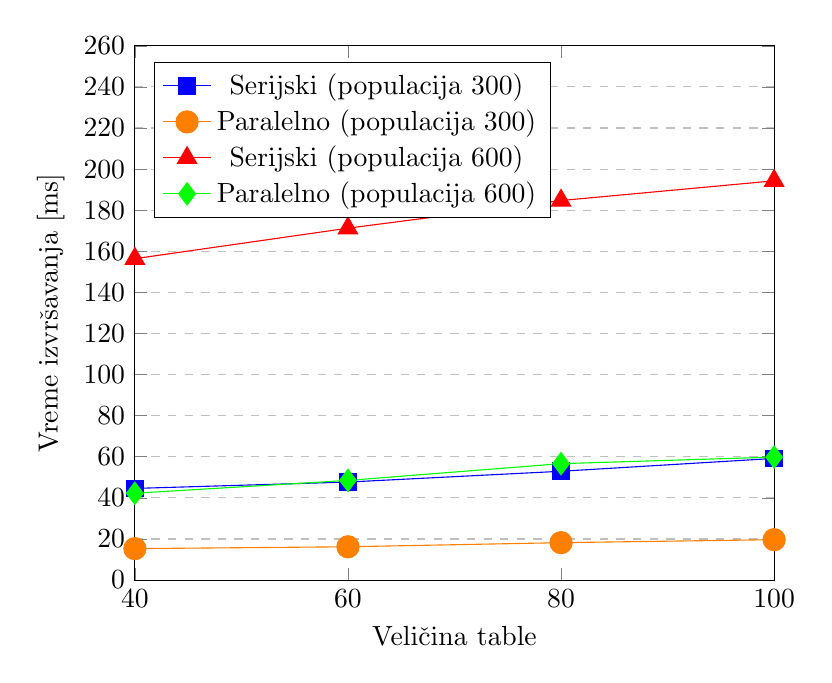
\begin{tikzpicture}
			\begin{axis}[
				width=0.8\textwidth,
				xlabel={Veličina table},
				ylabel={Vreme izvršavanja [ms]},
				xmin=40, xmax=100,
				ymin=0, ymax=260,
				xtick={40, 60, 80, 100},
				ytick={0,20,40,60,80,100,120,140,160,180,200,220,240,260},
				legend pos=north west,
				ymajorgrids=true,
				grid style=dashed,
				]
				
				\addplot[
				color=blue,
				mark=square*,
				mark size=3pt,
				]
				coordinates {
					(40, 44.6)(60, 47.7)(80, 52.95)(100, 59.2)
				};
				\addlegendentry{Serijski (populacija 300)}
				\addplot[
				color=orange, 
				mark=*,
				mark size=4pt
				]
				coordinates {
					(40, 15.3)(60, 16.2)(80, 18.2)(100, 19.65)
				};
				\addlegendentry{Paralelno (populacija 300)}
				\addplot[
				color=red,
				mark=triangle*,
				mark size=4pt,
				]
				coordinates {
					(40, 156.4)(60, 171.25)(80, 184.7)(100, 194.3)
				};
				\addlegendentry{Serijski (populacija 600)}
				\addplot[
				color=green, 
				mark=diamond*,
				mark size=4pt,
				]
				coordinates {
					(40, 42.25)(60, 48.5)(80, 56.65)(100, 59.85)
				};
				\addlegendentry{Paralelno (populacija 600)}
			\end{axis}
		\end{tikzpicture}
	\end{center}
	\begin{center}
		Grafik 1: Vreme izvršavanja algoritma, po generaciji, za različite veličine populacije, u zavisnosti od veličine šahovske table\\
	\end{center}
	\newpage

	\begin{center}
		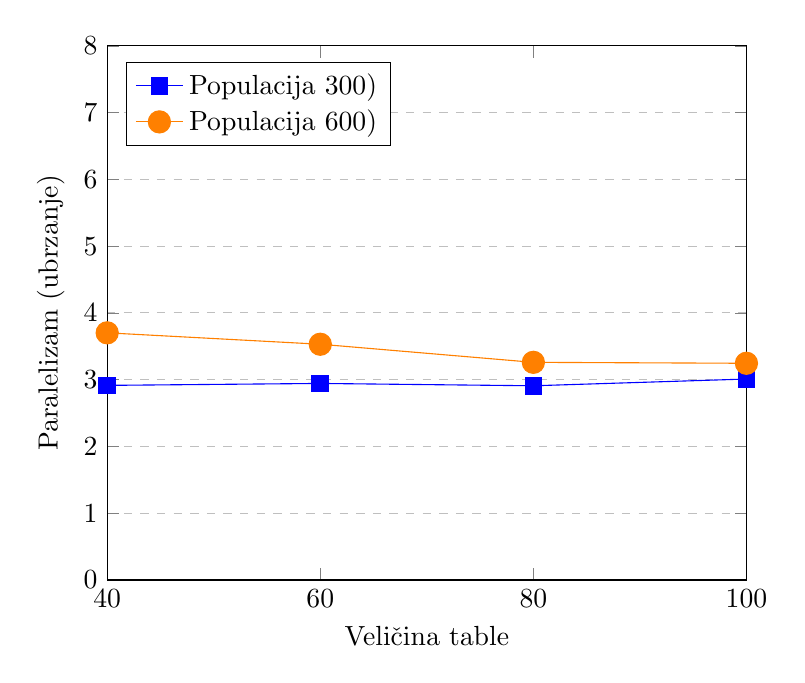
\begin{tikzpicture}
			\begin{axis}[
				width=0.8\textwidth,
				xlabel={Veličina table},
				ylabel={Paralelizam (ubrzanje)},
				xmin=40, xmax=100,
				ymin=0, ymax=8,
				xtick={40, 60, 80, 100},
				ytick={0,1,2,3,4,5,6,7,8},
				legend pos=north west,
				ymajorgrids=true,
				grid style=dashed,
				]
				
				\addplot[
				color=blue,
				mark=square*,
				mark size=3pt,
				]
				coordinates {
					(40, 2.915)(60, 2.944)(80, 2.909)(100, 3.01)
				};
				\addlegendentry{Populacija 300)}
				\addplot[
				color=orange, 
				mark=*,
				mark size=4pt
				]
				coordinates {
					(40, 3.702)(60, 3.531)(80, 3.260)(100, 3.246)
				};
				\addlegendentry{Populacija 600)}
			\end{axis}
		\end{tikzpicture}
	\end{center}
	\begin{center}
		Grafik 2: Ostvareni paralelizam (ubrzanje), za različite veličine populacije u zavisnosti od veličine šahovske table \\
	\end{center}

	\begin{center}
		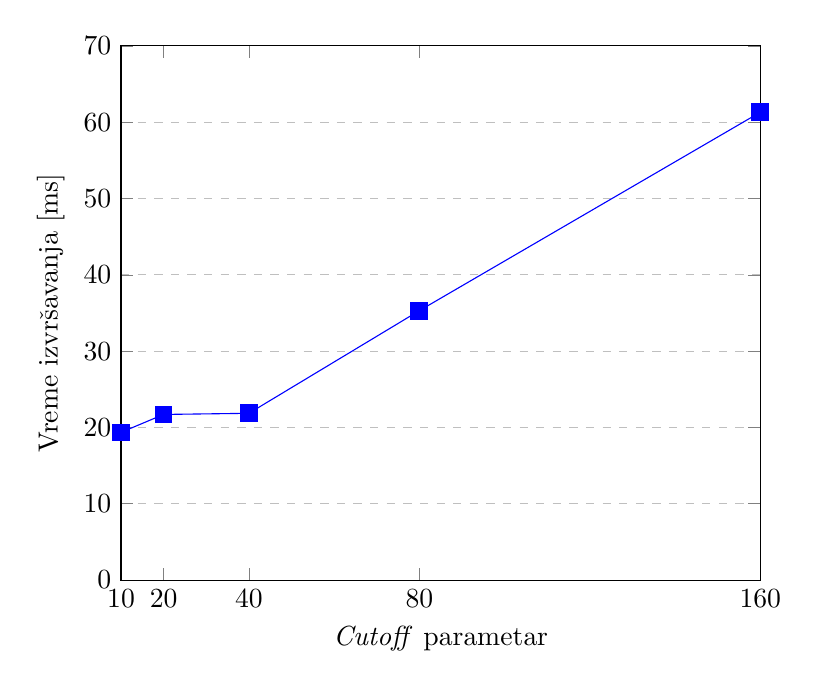
\begin{tikzpicture}
			\begin{axis}[
				width=0.8\textwidth,
				xlabel={\textit{Cutoff} parametar},
				ylabel={Vreme izvršavanja [ms]},
				xmin=10, xmax=160,
				ymin=0, ymax=70,
				xtick={10, 20, 40, 80, 160},
				ytick={0, 10, 20, 30, 40, 50, 60, 70},
				ymajorgrids=true,
				grid style=dashed,
				]
				
				\addplot[
				color=blue,
				mark=square*,
				mark size=3pt,
				]
				coordinates {
					(10, 19.35)(20, 21.7)(40, 21.85)(80, 35.3)(160, 61.3)
				};
			\end{axis}
		\end{tikzpicture}
	\end{center}
	\begin{center}
		Grafik 3: Vreme izvršavanja algoritma, po generaciji, za veličinu populacije 300 i veličinu šahovske table 100 u zavisnosti od \textit{cutoff} parametra (veličine grupe) \\
	\end{center}

	Primećeno je da za \textit{cutoff} parametar veći od 20, i veličine populacije i šahovske table koje odgovaraju onima sa prošlog grafika procesor nije dovoljno upošljen, tj. njegov load na svim jezgrima ne prelazi 90\%. Imajući to u vidu odlučili smo se da cutoff za date dimenzije bude 10, dok smo za ostale učestale dimenzije koristili druge vrednosti parametra, koje su se isto empirijski pokazale kao najbolje.
	
	\newpage
	
	\section{Zaključak}
	Kao što je i poznato, genetski algoritam nema garancije pronalaženja rešenja, a razlog te nepredvidljivosti su u velikoj meri mutacije i ukrštanja. Takođe, empirijskom proverom zaključeno je da program koji radi sa manjom kardinalnosti populacije brže konvergira ka traženom rešenju, prilikom serijskog izvršavanja. Paralelizacijom dobijamo mogućnost da povećamo veličinu populacije, čime trošimo više resursa, ali ukupno vreme izvršavanja je kraće.
	
	Paralelizacija programa pruža mogućnost efikasnijeg korišćenja dostupnih hardverskih resursa, što može rezultovati poboljšanjem performansi i smanjenjem vremena izvršavanja. Upotrebom odgovarajućih tehnika, moguće je rasporediti radne zadatke na više procesora ili jezgara i ostvariti istovremeno izvršavanje, čime se postiže ubrzanje izvršavanja. Ograničenja koja paralelizacija nosi su trke do podataka i veća kompleksnost koda, kao i teže otkrivanje grešaka. Pravilan odabir algoritama i strategija, kao i pažljivo upravljanje podacima i sinhronizaija istih predstavljaju ključne korake u postizanju optimalnih rezultata.
	
	Uprkos navedenim izazovima, paralelizacija se pokazuje kao snažan alat za poboljšanje performansi programa. Ispravno implementirana paralelizacija može doneti značajno kraće vreme izvršavanja, ali i bolju upotrebu raspoloživih resursa.
	
	\newpage
	
	\section{Tabele}
	
	\begin{center}
		\begin{tabular}{||c c c||} 
			\hline
			Veličina table & Serijski (populacija 300) [ms] & Paralelno (populacija 300) [ms] \\ [0.5ex] 
			\hline\hline
			40 & 44.6 & 15.3 \\ 
			\hline
			60 & 47.7 & 16.2 \\
			\hline
			80 & 52.95 & 18.2 \\
			\hline
			100 & 59.2 & 19.65 \\
			\hline
		\end{tabular}
	\end{center}
	\begin{center}
		Tabela 1: Tabela za grafik 1 (1. deo)
	\end{center}

	\begin{center}
		\begin{tabular}{||c c c||} 
			\hline
			Veličina table & Serijski (populacija 600) [ms] & Paralelno (populacija 600) [ms] \\ [0.5ex] 
			\hline\hline
			40 & 156.4 & 42.25 \\ 
			\hline
			60 & 171.25 & 48.5 \\
			\hline
			80 & 184.7 & 56.65 \\
			\hline
			100 & 194.3 & 59.85 \\
			\hline
		\end{tabular}
	\end{center}
	\begin{center}
		Tabela 2: Tabela za grafik 1 (2. deo)
	\end{center}

	\begin{center}
		\begin{tabular}{||c c c||} 
			\hline
			Veličina table & Populacija 300 & Populacija 600 \\ [0.5ex] 
			\hline\hline
			40 & 2.915 & 3.702 \\ 
			\hline
			60 & 2.944 & 3.531 \\
			\hline
			80 & 2.909 & 3.260 \\
			\hline
			100 & 3.01 & 3.246 \\
			\hline
		\end{tabular}
	\end{center}
	\begin{center}
		Tabela 3: Tabela za grafik 2
	\end{center}

	\begin{center}
		\begin{tabular}{||c c ||} 
			\hline
			\textit{Cutoff} & Vreme izvršavanja [ms]\\ [0.5ex] 
			\hline\hline
			10 & 19.35 \\ 
			\hline
			20 & 21.7 \\
			\hline
			40 & 21.85 \\
			\hline
			80 & 35.3 \\
			\hline
			100 & 61.3 \\
			\hline
		\end{tabular}
	\end{center}
	\begin{center}
		Tabela 4: Tabela za grafik 3
	\end{center}
		
	\end{document}
